\section{Transverse isotropic elasticity}

If the material properties are independent of orientations and directions of the technical or natural object under consideration, the material behavior is called {\sl isotropic}. Otherwise, the material is known as {\sl anisotropic} one. Anisotropy is closely connected with distinguished orientations in the material structure. Among others, fiber-reinforced and layered materials are typical anisotropic materials.

From the the point of view of modeling and numerical simulation special cases of anisotropy like {\sl orthotropy} are of particular interest. Orthotropic materials are characterized by mutually orthogonal two-fold axes of rotational symmetry. A special class of orthotropic materials represent the so called {\sl transverse isotropic} materials. They are characterized by a plane of isotropy featuring the same material properties independent of the direction of observation within this plane, and different material properties in the direction normal to this plane. Within this context, the normal to the plane of isotropy can be considered as the direction of anisotropy. Most of layered materials, biological membranes as well as rocks (e.\,g. sandstone, shale) are typical materials which can be considered as transverse isotropic ones.

In case of transverse isotropy, the Hooke's law (\ref{eq:hook}) has to be modified establishing a unit vector $\miu{a}{}{}$ which defines the direction perpendicular to the plane of isotropy (normal vector, direction of anisotropy -- defining, e.\,g., the direction of a single fiber family of a fiber-reinforced material).
\begin{eqnarray}
\sigma_{ij}& = & \lambda\,\delta_{ij}\,\varepsilon_{kk}\,+\,2\mu_T\,\varepsilon_{ij} \nonumber \\[1.50ex]
 &  & +\,2\,\left(\mu_L-\mu_T\right)\,\left(a_i\,\varepsilon_{jl}\,a_l+a_l\,\varepsilon_{li}\,a_j\right) 
 \nonumber \\[1.50ex]
 &  & +\,\alpha\,\left(a_i\,a_j\,\varepsilon_{kk}+a_k\,\varepsilon_{kl}\,a_l\,\delta_{ij}\right) 
 \nonumber \\[1.50ex]
 &  & +\,\beta\,a_k\,\varepsilon_{kl}\,a_l\,a_i\,a_j
\label{hooke_transviso}
\end{eqnarray}
Linear elastic transverse isotropic material is characterized by 5 independent material parameters like $\lambda$, $\mu_T$, $\mu_L$, $\alpha$ and $\beta$ given in Eqn. (\ref{hooke_transviso}). In some cases these parameters are called {\sl invariants} of the transverse isotropic elastic Hooke's law. They can be defined w.l.o.g. by the following (engineering) elastic constants which can be obtained experimentally: 

\begin{center}
\begin{tabular}{p{0.08\textwidth}p{0.025\textwidth}p{0.8\textwidth}}
$E_i$      & -- & Young's modulus within the plane of isotropy, \\[0.5ex]
$\nu_i$    & -- & Poisson's ratio within the plane of isotropy, \\[1.5ex]
$E_a$      & -- & Young's modulus w.r.t. the direction of anisotropy, \\[0.5ex]
$\nu_{ia},\,\nu_{ai}$ & -- & Poisson's ratio w.r.t. the direction of anisotropy, \\[0.5ex]
$G_a$      & -- & shear modulus w.r.t. the direction of anisotropy.
\end{tabular}
\end{center}

There exist some relations between these parameters.
\begin{eqnarray}
G_i      & \!\!\!\!\!= & 
\!\!\!\!\!\ttfrac{E_i}{2(1+\nu_i)}=\mu_i\;\;\mbox{(shear modulus within the plane of isotropy)} \\[2.0ex]
\nu_{ai} & \!\!\!\!\!= & \!\!\!\!\!\nu_{ia}\,\ttfrac{E_a}{E_i}
\end{eqnarray}

As mentioned above, the invariants of the transverse isotropic elastic Hooke's law can be expressed by the presented elastic parameters.
\begin{eqnarray*}
\lambda & = &  \ttfrac{E_i(\nu_i+\nu_{ia}\nu_{ai})}{{\widetilde D}} \\[2.0ex]
\mu_T   & = &  G_i \\[2.0ex]
\mu_L   & = &  G_a \\[2.0ex]
\alpha  & = &  \ttfrac{E_i(\nu_{ai}(1+\nu_i-\nu_{ia})-\nu_i)}{{\widetilde D}} \\[2.0ex]
\beta   & = &  \ttfrac{E_a(1-\nu_i^2)-E_i[(\nu_i+\nu_{ia}\nu_{ai})+2(\nu_{ai}(1+\nu_i-\nu_{ia})-\nu_i)]}
                      {{\widetilde D}} \\
        &   & \,-\,4G_a\,+\,2G_i \\[4.0ex]
        &   &  \mbox{with}\quad {\widetilde D}\,=\,
               1\,-\,\nu_i^2\,-\,2\,\nu_{ia}\,\nu_{ai}\,-\,2\,\nu_{ia}\,\nu_{i}\,\nu_{ai} \nonumber \\[1.0ex]
        &   &  \mbox{\hspace*{9.0ex}} =\,
               (1\,+\,\nu_i)(1\,-\,\nu_i\,-\,2\,\nu_{ia}\,\nu_{ai})
\end{eqnarray*}

The coordinates of the material tensor for linear elastic transverse isotropic material are defined as follows:
\begin{eqnarray}
\mathcal{C}_{ijkl} & = & \lambda\,\delta_{ij}\,\delta_{kl}\,+\,
                        2\mu_T\,\delta_{ik}\,\delta_{jl} \nonumber \\[1.50ex]
                   &   & +\,2\,\left(\mu_L-\mu_T\right)\,
                         \left(a_i\,\delta_{jk}\,a_l+a_k\,\delta_{il}\,a_j\right) \nonumber \\[1.50ex]
                   &   & +\,\alpha\,\left(a_i\,a_j\,\delta_{kl}+a_k\,a_l\,\delta_{ij}\right) \nonumber \\[1.50ex]
                   &   & +\,\beta\,a_i\,a_j\,a_k\,a_l
\end{eqnarray}

Tension of a quadratic plate according to Schr\"oder \cite{Schroeder:1996}, Kohlmeier \cite{Kohlmeier:2006} and Fiolka \cite{Fiolka:2007} is carried out to verify the linear elastic transverse isotropic material model. The model definition and the results are presented in the following examples.

\clearpage

\subsection{Tensile test (2D)}
\label{subsec:transiso_tens2d}
\subsubsection*{Problem definition}

The first example for transverse isotropic ellasticity is the twodimensional simplification of the tension of a quadratic plate under plane strain conditions according to Schr\"oder \cite{Schroeder:1996} and Kohlmeier \cite{Kohlmeier:2006}. Within this context, a laminated material structure perpendicular to the plane under consideration is assumed. The direction of anisotropy within this plane, which is defined by a vector $\miu{a}{}{}$ is perpendicularly oriented to the material layers. During simulation, the direction of anisotropy is rotated counterclockwise starting with an angle $\varphi$ of $\varphi=0^{\circ}$ and ending with $\varphi=180^{\circ}$. Consequently, as in {\sl OpenGeoSys} the direction of anisotropy is assumed to be directed parallel to the local $\bar{y}$-axis, and the angle of rotation is defined as the rotation between the global $x$-axis and the local $\bar{x}$-axis, the input angle changes in the range of $\varphi=-90^{\circ}$\dots$90^{\circ}$.

The quadratic plate has an edge length of $l=10\,$mm, and was analyzed using triangular and rectangular elements respectively. For details of the model (geometry, boundary conditions, material orientation) see Fig.~\ref{tens_transiso_model_2d}.

\begin{figure}[!htb]
\begin{center}
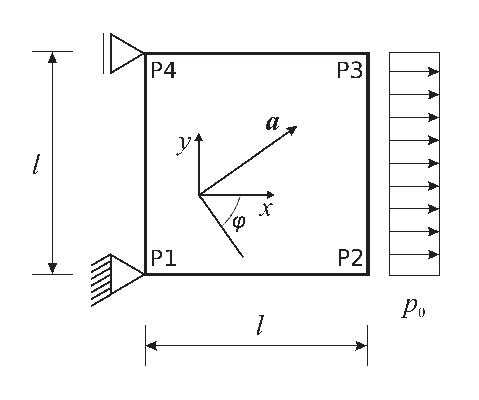
\includegraphics[scale=0.75]{M/figure/tenstest_model_mod.eps}
\end{center}
\caption{Tensile test. Model definition according to Kohlmeier \cite{Kohlmeier:2006}. Vector $\miu{a}{}{}$ defines the direction of anisotropy.}
\label{tens_transiso_model_2d}
\end{figure}

\subsubsection*{Initial and boundary conditions}

Initial conditions do not have to be given for the problem under consideration. The left-hand edge is fixed in horizontal direction. To avoid rigid body motions, the left lower corner node is fixed in both vertical and horizontal directions. A distributed tension load of $p_0=0.2\,$Mpa is applied at the right-hand edge. 

\subsubsection*{Material properties}

The material parameters are summarized in Tab.~\ref{matpar_transiso_tens}.

\begin{table}[!htb]
\centering
\begin{tabular}{lll}
\hline\hline\noalign{\smallskip}
Property & Value & Unit \\
\noalign{\smallskip}\hline\noalign{\smallskip}
Young's modulus $E_i$ & 561.12 & MPa \\
Young's modulus $E_a$ & 1311.83 & MPa \\
Poisson's ratio $\nu_i$ & 0.6032 & -- \\
Poisson's ratio $\nu_{ia}$ & 0.1838 & -- \\
shear modulus $G_a$ & 375.0 & MPa \\
\noalign{\smallskip}\hline\hline
\end{tabular}
\caption{Material parameters}
\label{matpar_transiso_tens}
\end{table}

\subsubsection*{Results}

The numerical results obtained with {\sl OpenGeoSys} are compared to values given in \cite{Kohlmeier:2006}. They include displacement coefficients of various corner nodes of the plate depending on the anisotropy direction, and show a good agreement (cf. Fig.~\ref{tens_transiso_test_2d}). 

\begin{figure}[!htb]
\begin{center}
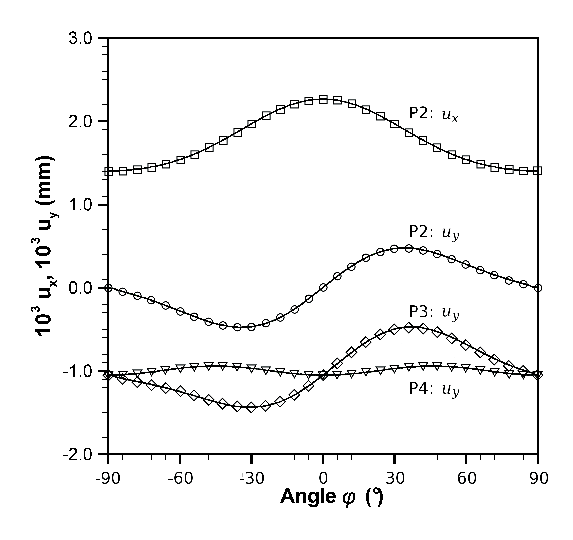
\includegraphics[scale=0.7]{M/figure/tenstest_results_OGS.eps}
\end{center}
\caption{Tensile test. {\sl OpenGeoSys} results (symbols) at length $l=10\,$mm and an edge load of $p_0=0.2\,$Mpa compared to the reference solution given by Schr\"oder \cite{Schroeder:1996} and Kohlmeier \cite{Kohlmeier:2006} (continuous lines).}
\label{tens_transiso_test_2d}
\end{figure}

\subsubsection*{Benchmark deposit}

\begin{tabular}{|l|l|l|}
  \hline
  Benchmark & Problem type & Path in benchmark deposit \\
  \hline
 \emph{m\_e\_transiso\_2D} & M & benchmarks\verb \M\ \\
  \hline
\end{tabular}



\clearpage

\subsection{Tensile test (3D)}
\label{subsec:transiso_tens3d}
\subsubsection*{Problem definition}

To verify the linear elastic transverse isotropic material model in the three dimensional case, the tensile test analyzed in Sec.~\ref{subsec:transiso_tens2d} was simulated using a rectangular sample with an edge length $l=10\,$mm and a height $h=1\,$mm. According to the twodimensional case, a vertically arranged laminated material structure is assumed. The direction of anisotropy, which is defined by a vector $\miu{a}{}{}$ is perpendicularly oriented to the material layers. During simulation, the direction of anisotropy is rotated counterclockwise in the $xy$-plane from $\varphi=0^{\circ}$ to $\varphi=180^{\circ}$. 

Within the context of the different opportunities offered by the input structure of {\sl OpenGeoSys} to define the anisotropy direction, the coefficients of the unit normal vector which is parallel to the direction of anisotropy are given as $n_x=\cos\varphi$, $n_y=\sin\varphi$, and $n_z=0$. Considering the case that the basis vectors of the local Cartesian coordinate system for transverse isotropic materials are provided by consecutive rotations of the plane of isotropy about the global $y$($x_2$)-axis and the $\bar{x}$($\bar{x}_1$)-axis of the once rotated system, the angle $\alpha$ has a constant value of $90^{\circ}$, whereas the angle $\beta$ changes from $0^{\circ}$ to $-180^{\circ}$. Using the angles known from applications in structural geology to generate the constitutive rotation matrices, the dip $\phi$ has the constant value of $90^{\circ}$, and the azimuth varies from $90^{\circ}$\dots$0^{\circ}$ (for $0^{\circ}\leq\varphi\leq 90^{\circ}$) and $360^{\circ}$\dots$270^{\circ}$ (for $90^{\circ}\leq\varphi\leq 180^{\circ}$) respectively.

For details of the model (geometry, boundary conditions, material orientation) see Fig.~\ref{tens_transiso_model_3d}.

\begin{figure}[!htb]
\begin{center}
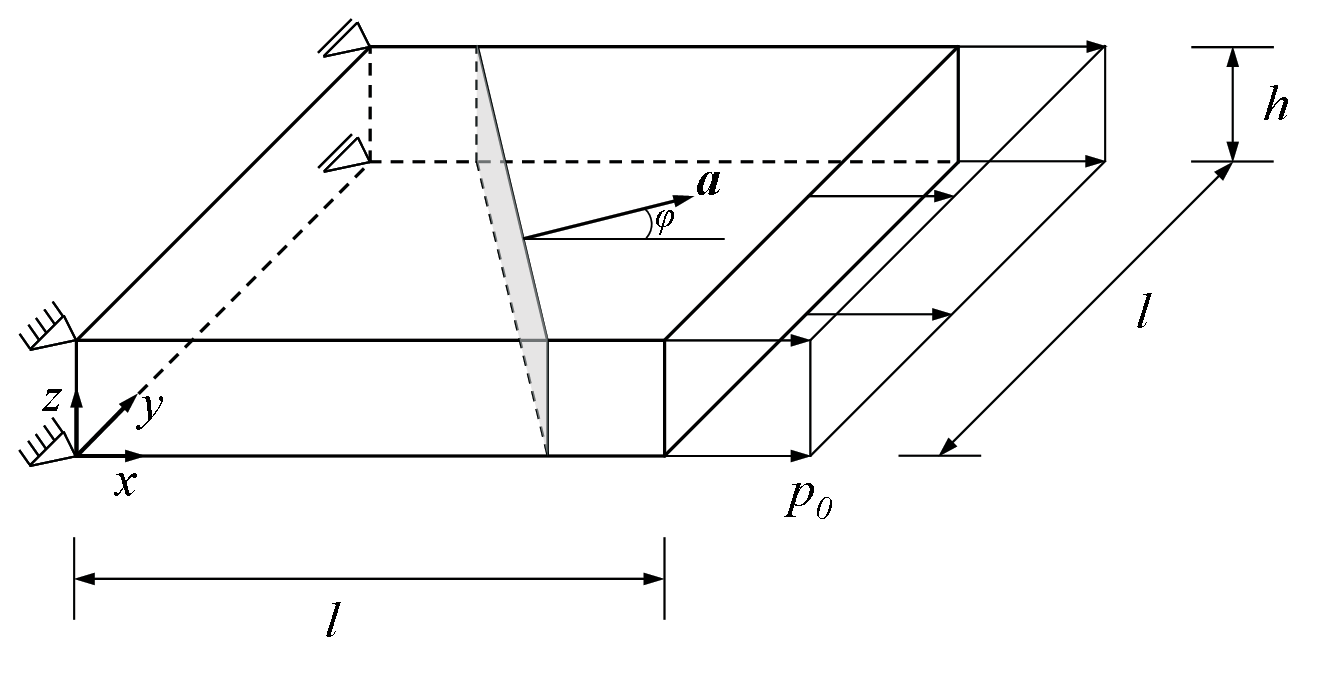
\includegraphics[width=0.7\textwidth]{M/figure/tenstest_model_3D.eps}
\end{center}
\caption{Tensile test. Threedimensional model definition according to Fiolka \cite{Fiolka:2007}. Vector $\miu{a}{}{}$ defines the direction of anisotropy.} 
\label{tens_transiso_model_3d}
\end{figure}

\subsubsection*{Initial and boundary conditions}

The initial and boundary conditions are the same as described for the two dimensional example  (cf. Sec.~\ref{subsec:transiso_tens2d}). The plane strain condition assumed for the twodimensional case was realized preventing any displacement in $z$-direction on the upper and lower boundary surfaces of the sample.

\subsubsection*{Material properties}

The material parameters are given in Tab.~\ref{matpar_transiso_tens}, as in the twodimensional case (cf. Sec.~\ref{subsec:transiso_tens2d}).

\subsubsection*{Results}

The results in the corresponding corner nodes of the sample are exactly the same as presented in Fig.~\ref{tens_transiso_test_2d} (cf. Sec.~\ref{subsec:transiso_tens2d}).

\subsubsection*{Benchmark deposit}

\begin{tabular}{|l|l|l|}
  \hline
  Benchmark & Problem type & Path in benchmark deposit \\
  \hline
 \emph{m\_e\_transiso\_3D} & M & benchmarks\verb \M\elasticity \\
  \hline
\end{tabular}


